\chapter{Methodology}

\section{Architectural Design Overview}

Red Sentinel is implemented using a microservice architecture. In this design, each major functional component of the system runs as an independent service. These services communicate via well-defined APIs and are coordinated by a central orchestration core the "Core Module." This microservice approach ensures that each module is isolated, independently deployable, testable, and can be scaled or replaced without impacting the rest of the system addressing concerns of maintainability, modularity, and system complexity typical in security tools.



\begin{figure}[H]
    \centering
    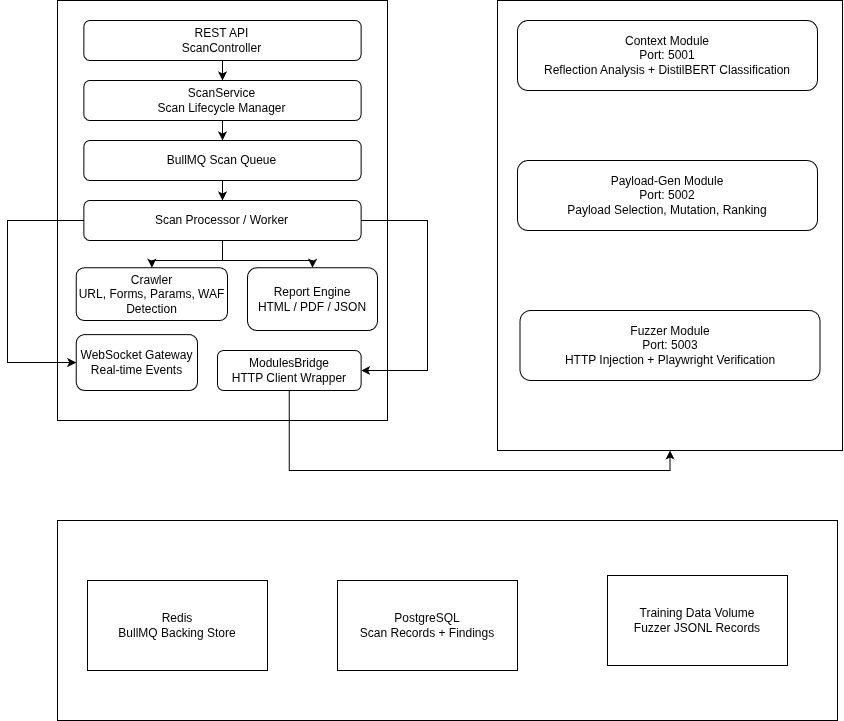
\includegraphics[width=1\linewidth]{figures/arch.png}
    \caption{System Architecture Diagram}
    \label{fig:system_architecture}
\end{figure}

The architecture consists of six primary services: a NestJS core service providing the REST API, WebSocket gateway, and job queue processor; three Python FastAPI microservices (Context, Payload-Gen, Fuzzer); a Next.js dashboard; and two infrastructure services (Redis and PostgreSQL).

\subsection{Design Principles}
\subsubsection{Separation of Concerns}

Each microservice is responsible for a single phase of the scanning pipeline. The Context module understands the injection context, the Payload Generation module understands payload selection and mutation, the Fuzzifier module understands HTTP-level injection and browser verification. The Core co-ordinates these phases without containing their implementation logic. This separation allows each service to be modified independently and be tested in isolation.

\subsubsection{Asynchronous Job Processing}
Scan jobs are not processed synchronously in the HTTP request-response cycle. When a client submits a POST /scan request, the Core immediately persists the scan record to PostgreSQL, enqueues a BullMQ job, and returns the scan ID to the client. The actual scanning pipeline executes asynchronously in a BullMQ worker process. This design decouples request handling from compute intensive scanning, allows multiple scans to be queued without blocking, and supports scan cancellation, retries, and priority management.

\subsubsection{Event-Driven Real-Time Updates}

The BullMQ scan processor emits events at each pipeline phase transition and upon each vulnerability discovery. These events are relayed to the NestJS WebSocket Gateway, which broadcasts them to subscribed Socket.io clients. This event-driven architecture provides clients with sub-second latency updates without polling.

\subsubsection{Health-Check Dependency Management}

Docker Compose service startup is conditioned on health checks: the Core service will not start until Redis, PostgreSQL, and all three Python microservices report healthy. Each Python service exposes a /health endpoint returning service status and model load state. This prevents race conditions during cold starts where the Core might attempt to call Python services before their AI models have loaded.

\subsection{Data Flow in Scan Execution}
A complete scan execution follows this data flow:
\begin{enumerate}[itemsep=2pt, topsep=-15pt]
    \item Client submits POST /scan with target URL, scan depth, and options.
    \item ScanController validates request, persists ScanRecord to PostgreSQL with status PENDING, enqueues BullMQ job with scan ID.
    \item  BullMQ Processor picks up job, updates status to RUNNING, begins Phase 1: CRAWL.
    \item Crawler spiders target URL up to configured depth, collecting all discovered URLs, query parameters, form fields, headers, and cookies. WAF detection heuristics run concurrently.
    Example:
      \begin{Verbatim}[fontsize=\scriptsize]
       Dicovered page:
        <script>
            var searchTerm = "USER_INPUT";
          </script>

                    Crawler output:
                    {
              "url": "https://demo-app.com/search?q=test",
              "parameter": "q",
              "reflectionPoint": "script_tag"}
      \end{Verbatim}
    \item Crawler results are passed to ModulesBridge, which issues POST /analyze to Context module (:5001).
    \item Context module probes each injection point with probe strings, analyzes reflections, and classifies each injection point's context using DistilBERT.
    \item Context classification results are passed to ModulesBridge, which issues POST /generate to Payload-Gen module (:5002).
    \item Payload-Gen module selects candidates from the dataset filtered by context, applies mutation and obfuscation, ranks payloads using a secondary ranker model.
     Example:
      \begin{Verbatim}[fontsize=\scriptsize]
       {
          {    "payloads": [
                "\";alert(1);//",
                "\"};alert(document.domain);//",
               ..........
              ]
            }
      \end{Verbatim}
    \item Ranked payloads are passed to ModulesBridge, which issues POST /fuzz to Fuzzer module (:5003).
    \item  Fuzzer injects payloads, checks HTTP responses for reflection, launches Playwright headless browser for verification of apparent reflections. Confirmed executions are reported as vulnerabilities.  Example:
      \begin{Verbatim}[fontsize=\scriptsize]
       {
          Injected response:
                <script>
        var searchTerm = "";alert(1);//";
      </script>
            }
      \end{Verbatim}
    \item Report Engine generates HTML/PDF/JSON reports. Scan status is set to COMPLETED. scan:complete WebSocket event is broadcast.
\end{enumerate}
\newpage
\begin{figure}[h]
  \centering
  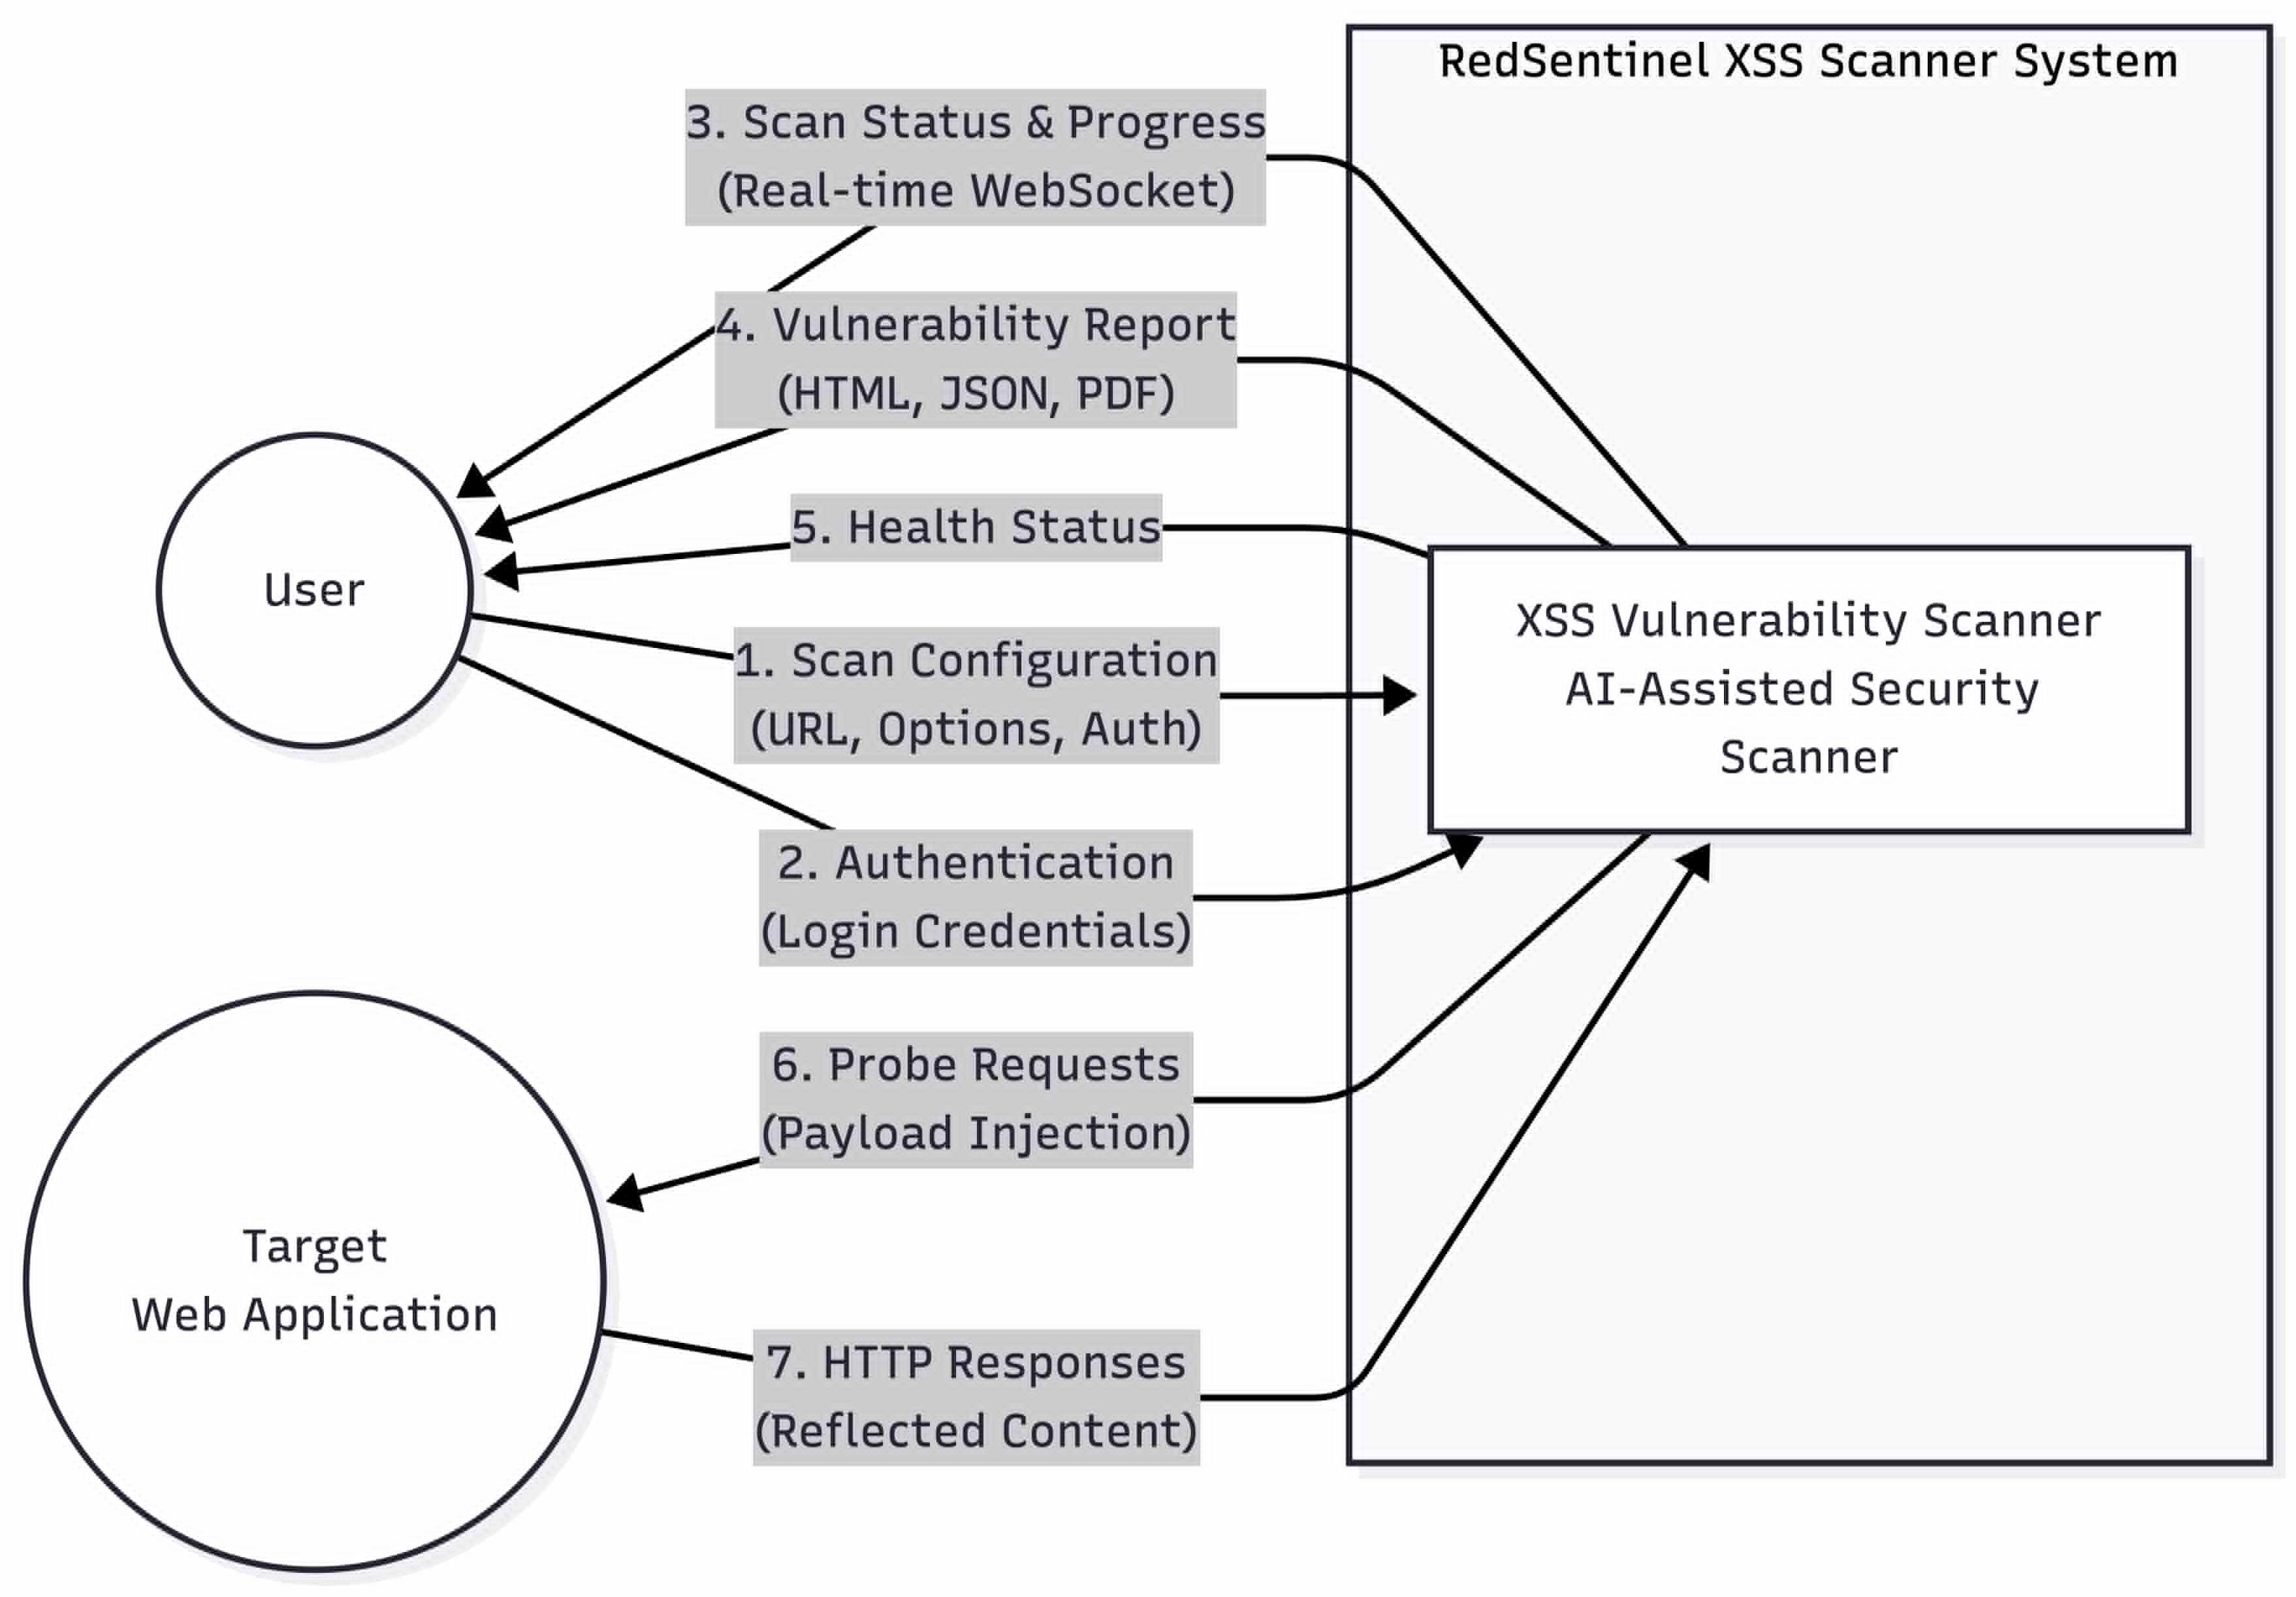
\includegraphics[width=0.8\textwidth]{figures/DFD0.jpg}
  \caption{High-Level Architecture and Communication Flow of the RedSentinel AI-Assisted XSS Vulnerability Scanner System.}
  \label{fig:example_image}
\end{figure}

\begin{figure}[H]
  \centering
  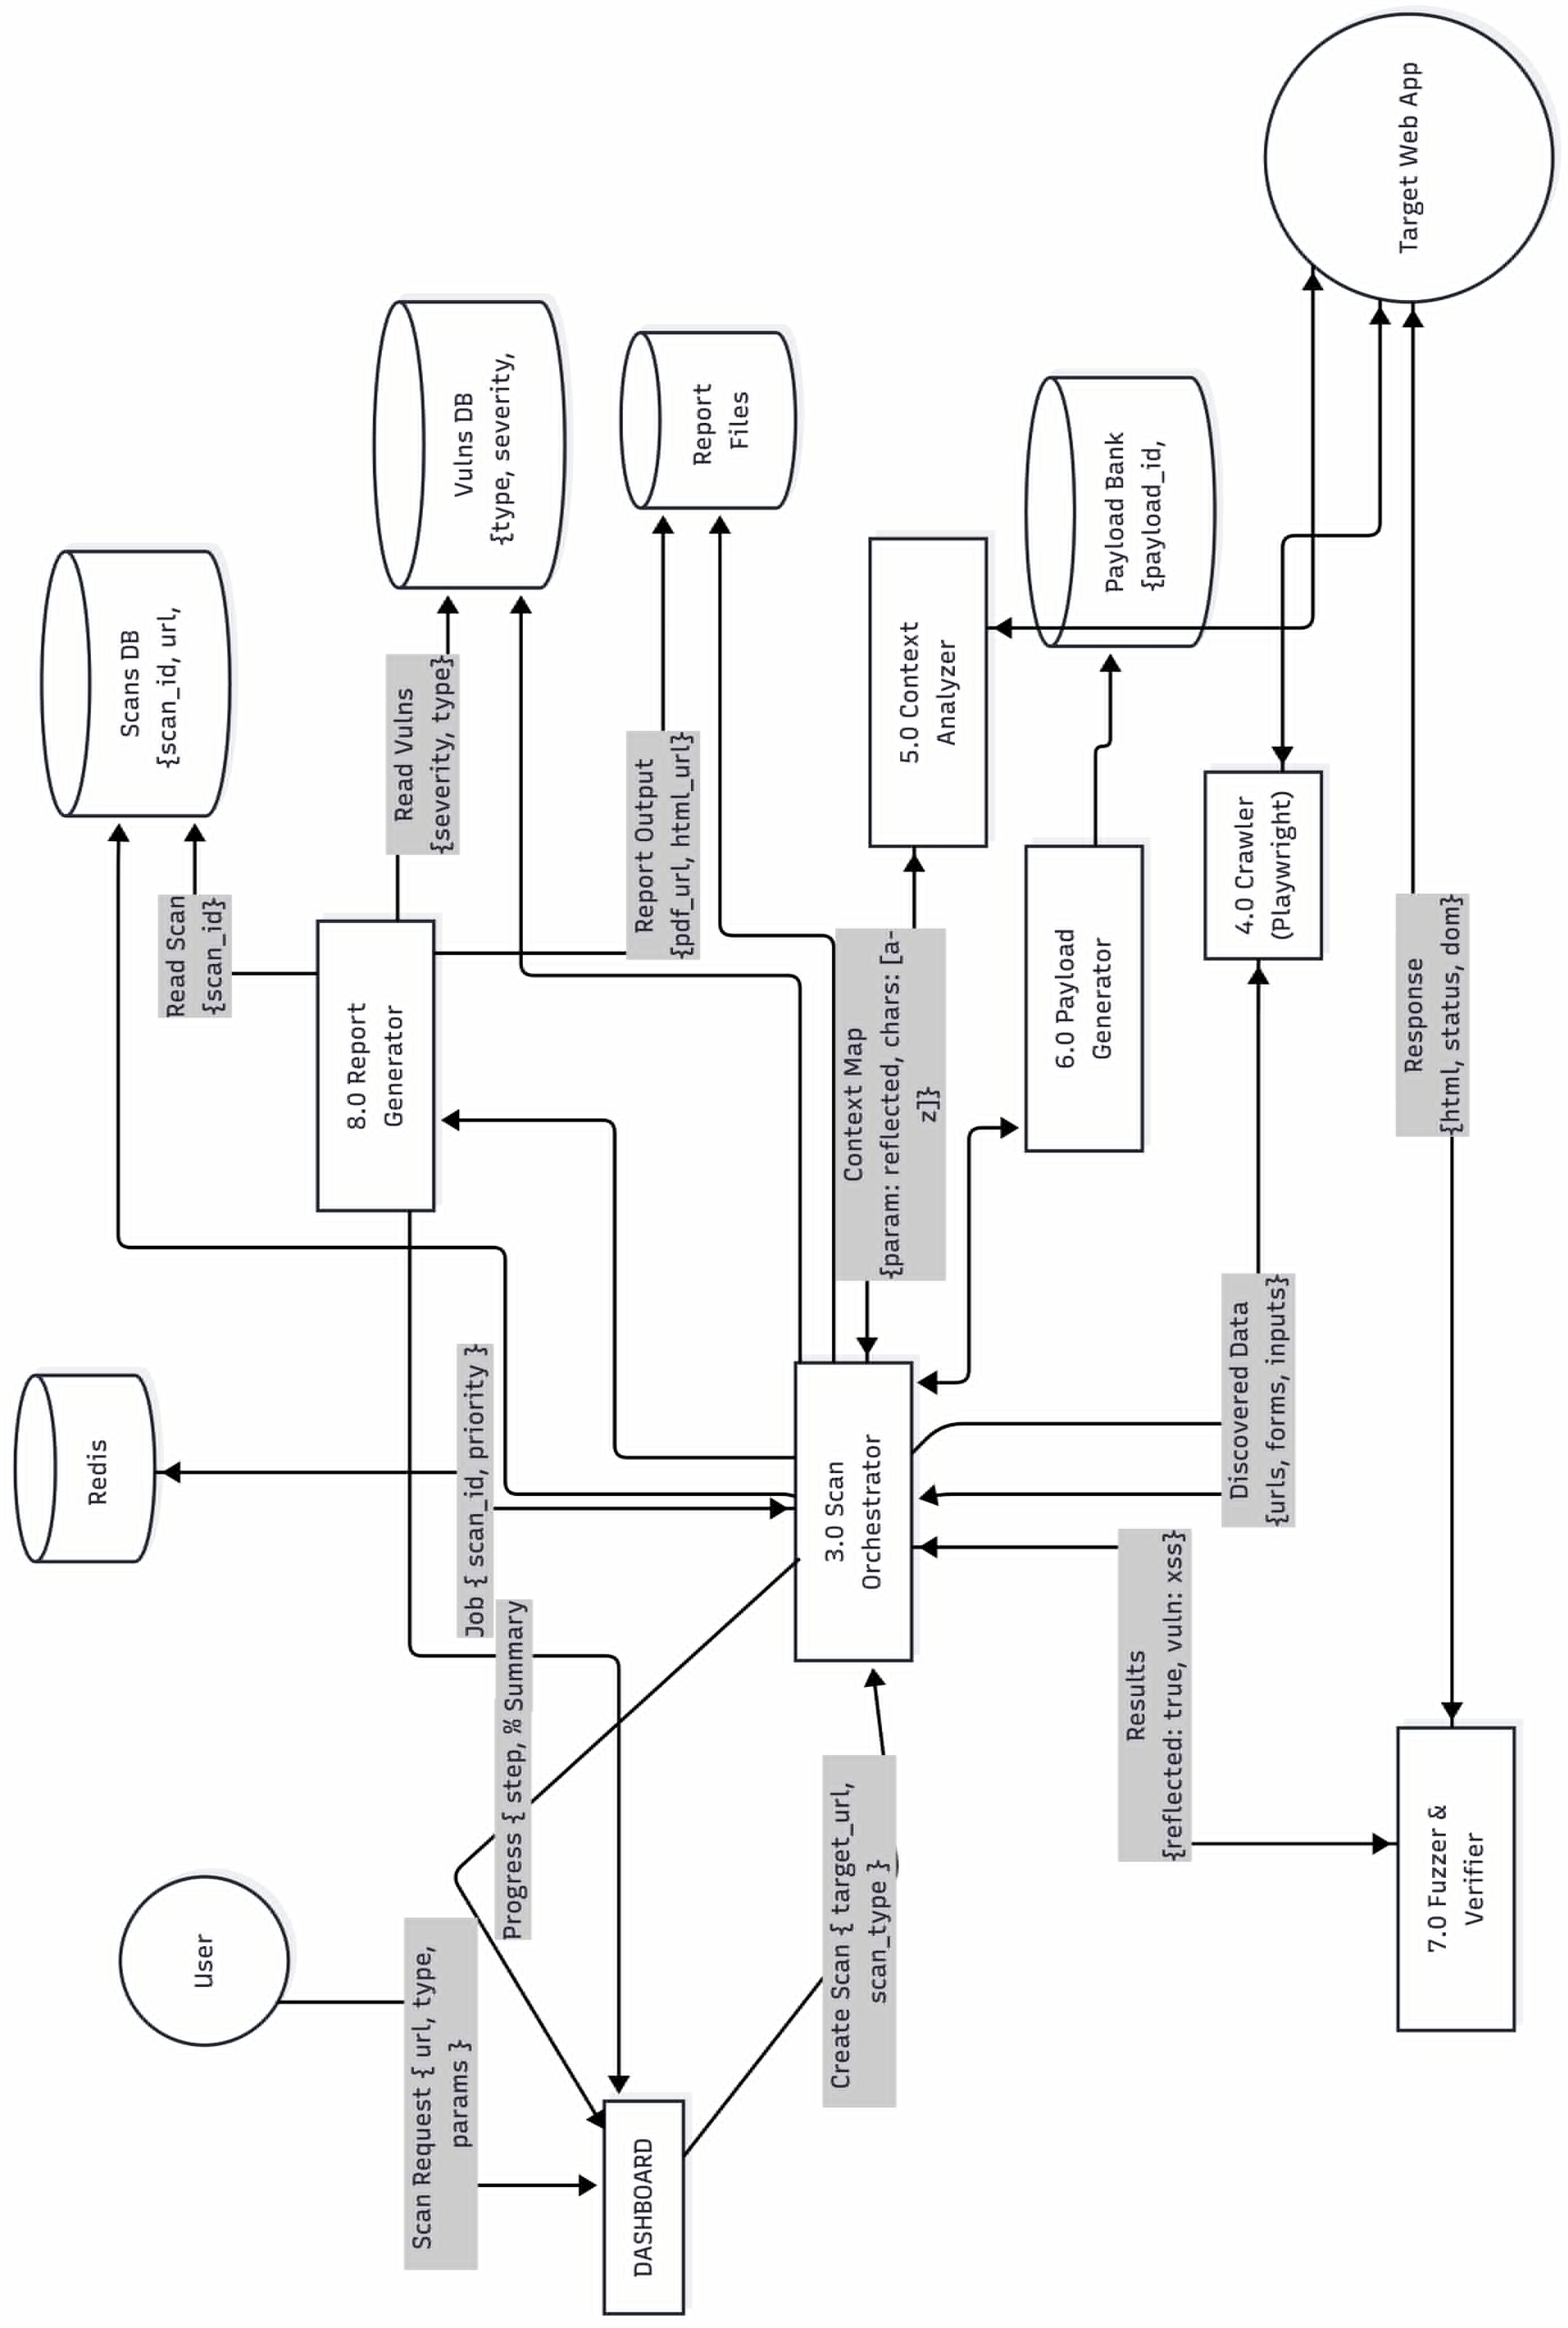
\includegraphics[angle=-90,width=1\textwidth]{figures/dfd1.jpg}
  \caption{Detailed System Architecture and Data Flow of the RedSentinel AI-Assisted XSS Scanning Framework}
  \label{fig:example_image}  
\end{figure}

\newpage
\subsection{Tech stack}
    \renewcommand{\arraystretch}{1.5}


\begin{table}[H]
    \centering
    \begin{tabular}{|p{2.7cm}|p{3cm}|p{8cm}|}
    \hline
    \textbf{Layer} &
    \textbf{Technology} &
    \textbf{Rationale} \\
    \hline
    
    Core API &
    NestJS (TypeScript) &
    Dependency injection, modular architecture, built-in validation, Swagger generation, first-class WebSocket support \\
    \hline
    
    Job Queue &
    BullMQ + Redis &
    Reliable job delivery with at-least-once semantics, priority queues, job cancellation, delayed retries, dashboard monitoring \\
    \hline
    
    AI / Security Modules &
    Python 3.11 + FastAPI &
    PyTorch/HuggingFace ecosystem for transformer models; Playwright for headless browser; Pydantic for schema validation \\
    \hline
    
    AI Model &
    DistilBERT (HuggingFace) &
    97\% of BERT accuracy at 40\% fewer parameters; fast inference suitable for scan pipeline latency requirements \\
    \hline
    
    Frontend &
    Next.js 16 + Tailwind CSS 4 &
    Server components for initial render; Socket.io client for real-time updates; Tailwind for utility-first styling \\
    \hline
    
    Database &
    PostgreSQL 16 &
    ACID compliance; jsonb columns for flexible vulnerability metadata; reliable with read-heavy workloads \\
    \hline
    
    Report Generation &
    Handlebars + Puppeteer &
    Handlebars templates for structured HTML reports; Puppeteer renders HTML to high-fidelity PDF \\
    \hline
    
    Containerization &
    Docker Compose &
    Service isolation; deterministic builds; health-check-based startup ordering; volume management for persistent data \\
    \hline
    \end{tabular}
    \caption{Technology Stack Rationale}
    
\end{table}
\section{Module Design and Implementation}
\subsection{NestJS Core Service}
\subsubsection{Module Section}
The NestJS core is organized into seven modules following NestJS's opinionated module system.
Each module encapsulates its own controllers, services, and test files.
   \begin{table}[H]
    \centering
    \begin{tabular}{|p{2.7cm}|p{5cm}|p{4cm}|}
    \hline
    \textbf{Module} &
    \textbf{Responsibility} &
    \textbf{Key Classes} \\
    \hline
    
    ScanModule &
    Scan CRUD operations, lifecycle management, WebSocket event emission &
    ScanController, ScanService, ScanGateway \\
    \hline
    
    QueueModule &
    BullMQ job production and consumption; pipeline orchestration &
    ScanProducer, ScanProcessor \\
    \hline
    
    ReportModule &
    HTML/PDF/JSON report generation and file management &
    ReportService, ReportController \\
    \hline
    
    ModulesBridge Module &
    HTTP client wrappers for all three Python services &
    ContextClient, PayloadGenClient, FuzzerClient \\
    \hline
    
    AuthModule &
    API key extraction and validation guard &
    ApiKeyGuard, AuthService \\
    \hline
    
    HealthModule &
    Aggregated health check endpoint polling all dependencies &
    HealthController, PythonHealthIndicator \\
    \hline
    
    CommonModule &
    Shared interfaces, exception filters, utility functions &
    GlobalExceptionFilter, ValidationPipe \\
    \hline
    \end{tabular}
    \caption{NestJS Core Module Structure}
    \end{table}
\subsubsection{Scan Module}
\subsubsection{ Scan Controller and Service}
The ScanController exposes the public REST API surface, delegating all business logic to ScanService. Controller methods are thin: they validate incoming DTOs using class-validator decorators, call ScanService, and return HTTP responses. The ScanService is responsible for:
\begin{itemize}[itemsep=2pt, topsep=-15pt]
    \item Persisting new scan records to PostgreSQL via TypeORM repositories.
    \item Enqueuing scan jobs to BullMQ via ScanProducer.
    \item Retrieving scan status and vulnerability lists for GET endpoints.
    \item Handling scan cancellation by removing the BullMQ job and updating scan status
    \item Providing paginated scan listing with sorting and filtering capabilities. 
\end{itemize}
\subsubsection{ BullMQ Queue Architecture}
BullMQ is a Redis-backed job queue library for Node.js. RedSentinel uses a single 'scan-queue' with the following configuration:
\begin{itemize}[itemsep=2pt, topsep=-15pt]
    \item Concurrency: 2 simultaneous scan jobs per worker instance (configurable). This prevents memory exhaustion from concurrent Playwright browser instances.
    \item Retry policy: Up to 3 retries with exponential backoff starting at 5 seconds. Scan jobs that fail after all retries are moved to a failed state and the scan record is updated accordingly.
    \item Job timeout: 60,000 ms default (configurable via DEFAULT\_\allowbreak TIMEOUT\_\allowbreak MS). Long-running scans against large targets require extended timeouts.
    \item Job removal: Completed jobs are removed after 24 hours. Failed jobs are retained for 7 days for post-mortem debugging.
\end{itemize}

\textbf{M/G/c Queue Model}

Scan requests arrive as a Poisson process with rate $\lambda$ (arrivals/sec). Each scan has a generally distributed service time $S$ with mean $
\mathbb{E}[S] = \frac{1}{\mu}
$
and second moment
$ \mathbb{E}[S^2].$
The system has $c$ concurrent worker processes. Under these assumptions:
\subparagraph*{Traffic Intensity per Server}

\[
\rho = \frac{\lambda}{c\mu}
\]

\subparagraph*{Stability Condition}

\[
\rho < 1
\iff
\lambda < c\mu
\]

\subparagraph*{Pollaczek--Khinchine Mean Waiting Time (M/G/1 Baseline)}

\[
W_q =
\frac{\lambda \, \mathbb{E}[S^2]}
     {2(1-\rho)}
\]

\subparagraph*{Coefficient of Variation}

\[
C_v =
\frac{\sqrt{\mathrm{Var}[S]}}
     {\mathbb{E}[S]}
\]

\subparagraph*{M/G/c Kingman Approximation}

\[
W_q \approx
\frac{C_v^2 + 1}{2}
\cdot
\frac{\rho^{\sqrt{2(c+1)} - 1}}
     {c(1-\rho)}
\cdot
\mathbb{E}[S]
\]

This gives system operators a formula to tune
\texttt{DEFAULT\_MAX\_PAYLOADS}
and concurrency $c$ to meet a target P99 scan latency SLA, without violating Redis memory pressure bounds.


\subsubsection{WebSocket Gateway}
The ScanGateway implements the Socket.io server using NestJS's @WebSocketGateway decorator. Clients subscribe to scan-specific rooms identified by scan ID. The gateway emits four
event types:

\begin{table}[h]
\centering
\renewcommand{\arraystretch}{1.5}
\begin{tabular}{|p{3cm}|p{6cm}|p{4cm}|}
\hline
\textbf{Event} &
\textbf{Payload} &
\textbf{Trigger} \\
\hline

scan:progress &
\{ scanId, phase, progress, message \} &
Each pipeline phase transition; progress percentage updates \\
\hline

scan:finding &
\{ scanId, vulnerability: VulnerabilityDto \} &
Each confirmed XSS finding during fuzzing phase \\
\hline

scan:complete &
\{ scanId, summary: ScanSummaryDto \} &
Scan pipeline completion (success) \\
\hline

scan:error &
\{ scanId, error: string \} &
Unrecoverable scan failure after retries exhausted \\
\hline

\end{tabular}
\caption{WebSocket Gateway Event Types}
\end{table}

\subparagraph*{WebSocket Progress as a Continuous-Time Markov Chain}

The 5-phase scan pipeline\\
$
\texttt{CRAWL}
\rightarrow
\texttt{CONTEXT}
\rightarrow
\texttt{PAYLOAD\mbox{-}GEN}
\rightarrow
\texttt{FUZZ}
\rightarrow
\texttt{REPORT}
$ \\
can be modeled as a Continuous-Time Markov Chain (CTMC) to derive the expected completion time and phase-conditional progress distributions.

\subparagraph*{State Space}
$
S =
\{
0=\texttt{IDLE},
1=\texttt{CRAWL},
2=\texttt{CONTEXT},
3=\texttt{PAYLOAD\mbox{-}GEN},
4=\texttt{FUZZ},
5=\texttt{REPORT},
6=\texttt{DONE}
\}
$

\subparagraph*{Generator Matrix}

Let, $ Q \in \mathbb{R}^{7 \times 7} $denote the CTMC generator matrix, defined by:

\[
Q_{ii} = -\mu_i,
\qquad
Q_{i,i+1} = \mu_i
\quad
\text{for \{} i=0,\dots,5 
\text{\}}
\quad
\text{ and } 
\quad
Q_{6j} = 0 
\]

where state \(6\) is an absorbing state corresponding to scan completion.

\subparagraph*{Expected Scan Completion Time}

The expected remaining completion time starting from phase \(i\) is:

\[
\mathbb{E}[T_{\text{total}} \mid \text{phase}=i]
=
\sum_{k=i}^{5}
\frac{1}{\mu_k}
\]

\subparagraph*{Conditional Progress Distribution}

The probability of being in phase \(k\) at time \(t\) is:

\[
p_k(t)
=
\Pr(\text{phase}=k \text{ at time } t)
=
\left[e^{Qt}\right]_{0,k}
\]

where \(e^{Qt}\) denotes the matrix exponential of the generator matrix.

The WebSocket event
\texttt{scan:progress}
broadcasts the empirical phase index \(k\) and the fraction of payloads processed within phase \(4\) (\texttt{FUZZ}), providing users with a fine-grained real-time estimate of \(p_k(t)\).

\subsubsection{Report Engine}
The ReportService uses Handlebars templates to render HTML reports from scan data, then employs Puppeteer to render the HTML to PDF. The report engine supports three output formats HTML, PDF and JSON.
\subparagraph*{Vulnerability Scoring via CVSS and Formal Risk Calculus}
The report engine assigns a severity score to each discovered XSS vulnerability. This section derives the scoring formally, grounding the CVSS v3.1 base score in a utility-theoretic risk model.
\subparagraph*{CVSS v3.1 Base Score Formula}
\subparagraph*{CVSS Base Score Computation}

CVSS assigns numeric sub-scores to the following security metrics:

\[
\text{AV},\;
\text{AC},\;
\text{PR},\;
\text{UI},\;
\text{S},\;
\text{C},\;
\text{I},\;
\text{A}
\]

where:

\begin{itemize}
    \item AV = Attack Vector
    \item AC = Attack Complexity
    \item PR = Privileges Required
    \item UI = User Interaction
    \item S = Scope
    \item C = Confidentiality Impact
    \item I = Integrity Impact
    \item A = Availability Impact
\end{itemize}

\subparagraph*{Impact Sub-score}

The Impact Sub-score Base is defined as:


$ \mathrm{ISCBase}
=
1
-
(1-\mathrm{ImpactConf})
(1-\mathrm{ImpactInteg})
(1-\mathrm{ImpactAvail})$


The final impact score is:

\[
\mathrm{ISC}
=
\begin{cases}
6.42 \cdot \mathrm{ISCBase},
& \text{if Scope = UNCHANGED}
\\[1em]
7.52(\mathrm{ISCBase}-0.029)
-
3.25(\mathrm{ISCBase}-0.02)^{15},
& \text{if Scope = CHANGED}
\end{cases}
\]

\subparagraph*{Exploitability Sub-score}

\[
\mathrm{Exploitability}
=
8.22
\cdot
\mathrm{AV}
\cdot
\mathrm{AC}
\cdot
\mathrm{PR}
\cdot
\mathrm{UI}
\]

\subparagraph*{Base Score}

\[
\mathrm{Base}
=
\begin{cases}
0,
& \text{if } \mathrm{ISC} \le 0
\\[1em]
\mathrm{Roundup}
\left(
\min(\mathrm{ISC}+\mathrm{Exploitability},\,10)
\right),
& \text{if Scope = UNCHANGED}
\\[1em]
\mathrm{Roundup}
\left(
\min(1.08(\mathrm{ISC}+\mathrm{Exploitability}),\,10)
\right),
& \text{if Scope = CHANGED}
\end{cases}
\]

where \(\mathrm{Roundup}(\cdot)\) rounds to one decimal place toward positive infinity.

\subparagraph*{Example: Reflected XSS}

For reflected XSS (the primary target of RedSentinel), the typical CVSS metric values are:


$
\mathrm{AV} : N  (0.85)\text{, } 
\mathrm{AC} : L  (0.77) \text{, }
\mathrm{PR} : N  (0.85) \text{, }
\mathrm{UI} : R  (0.62) \text{, }
\mathrm{S}  : C \text{, }
\mathrm{C}  : L  (0.22)
\text{, } \quad
\mathrm{I}  : L  (0.22)\text{, }
\mathrm{A}  : N  (0.00)\text{, }
$


yielding a Base Score of approximately: $\mathrm{Base} \approx 6.1$ corresponding to a \texttt{MEDIUM} severity classification.
\subparagraph*{Expected Loss Model}
Beyond CVSS, the report engine can expose an expected monetary loss model. Given an asset value $V_asset$, an annualised attack frequency $\lambda_a$, and the CVSS-derived probability of successful exploit $P_exploit$:

\subparagraph*{Expected Loss and Annual Loss Expectancy}

The expected loss (\(\mathrm{EL}\)) from a vulnerability can be modeled as:

\[
\mathrm{EL}
=
\lambda_a
\cdot
P_{\mathrm{exploit}}
\cdot
V_{\mathrm{asset}}
\cdot
(1-\mathrm{control}_{\mathrm{effectiveness}})
\]

where:

\begin{itemize}
    \item \(\lambda_a\) = attack arrival rate
    \item \(P_{\mathrm{exploit}}\) = probability of successful exploitation
    \item \(V_{\mathrm{asset}}\) = asset value or potential loss magnitude
    \item \(\mathrm{control}_{\mathrm{effectiveness}}\) = effectiveness of deployed security controls
\end{itemize}

\subparagraph*{Exploit Probability Approximation}

The exploit probability is approximated from the CVSS exploitability score:

\[
P_{\mathrm{exploit}}
\approx
\frac{\mathrm{Exploitability}}{10}
\]

which normalizes the CVSS exploitability metric into the range \([0,1]\).

\subparagraph*{Annual Loss Expectancy (ALE)}

The Annual Loss Expectancy is defined as:

\[
\mathrm{ALE}
=
\frac{
\mathrm{EL} \cdot 365
}{
\mathrm{MTTR}
}
\qquad
\text{
where, 
 $\mathrm{MTTR}$ = Mean Time To Remediate (days)}
 \]

\subparagraph*{Risk Reduction from Patching}

The reduction in annualized risk after remediation is:

\[
\Delta \mathrm{ALE}
=
\mathrm{ALE}_{\mathrm{before}}
-
\mathrm{ALE}_{\mathrm{after}}
\]

Assuming successful patching eliminates exploitability,  $ P_{\mathrm{exploit}} \to 0 $ then: $\mathrm{ALE}_{\mathrm{after}} \to 0$ 
 
\[ \therefore \Delta \mathrm{ALE} = \mathrm{ALE}_{\mathrm{before}}\]

meaning the full expected annualized loss associated with the vulnerability is removed after remediation.
\subsection{ Context Module (Python :5001)}

The Context module is responsible for the second phase of the scan pipeline: analyzing each injection point discovered by the crawler to determine the XSS injection context. This is the AI intensive component of the system.
\subsubsection{API Contract}
The module exposes a FastAPI application with the following primary endpoints:
\begin{table}[h]
\centering
\renewcommand{\arraystretch}{1.2}
\begin{tabularx}{\textwidth}{|>{\raggedright\arraybackslash}p{2cm}|>{\raggedright\arraybackslash}p{5.5cm}|X|}
\hline
\textbf{Method} & \textbf{Endpoint} & \textbf{Behavior} \\
\hline

POST & \texttt{/scan} & Create a scan, enqueue it, and return the scan record \\
\hline

GET & \texttt{/scan/:id} & Return scan status and persisted vulnerabilities \\
\hline

GET & \texttt{/scans?page=\&limit=} & Return paginated scan records \\
\hline

GET & \texttt{/scan/:id/audit} & Return scan audit logs \\
\hline

GET & \texttt{/scan/:id/report} & Return \texttt{\{ reportUrl: "/reports/<id>.html" \}}; this is a pointer only \\
\hline

DELETE & \texttt{/scan/:id} & Cancel an active scan \\
\hline

DELETE & \texttt{/scans/:id} & Permanently delete one scan and its results \\
\hline

DELETE & \texttt{/scans} & Delete all scans, results, and reports \\
\hline

GET & \texttt{/reports/:scanId} & List available generated report formats and download links \\
\hline

GET & \texttt{/reports/:scanId/ ?format=html|json|pdf} & Download an existing report file \\
\hline

GET & \texttt{/reports/:scanId/ ?formats=html,json,pdf} & Regenerate selected report formats \\
\hline

GET & \texttt{/health} & Return aggregate health status \\
\hline

\end{tabularx}
\caption{Core Scan and Report API Routes}
\label{tab:scan-report-routes}
\end{table}


\subsubsection{Reflection Analysis}
Before invoking the AI classifier, the Context module performs HTTP-level reflection analysis. For each injection point, a set of probe strings are injected: a unique random alphanumeric string, an HTML tag probe (<xss-probe>), and a JavaScript probe ('<script>). The HTTP response is analyzed to determine:
\begin{itemize}
    \item Whether the probe string appears in the response body (reflection detection).
    \item The surrounding HTML context of the reflected string (parsed using BeautifulSoup).
    \item Whether the probe appears inside an HTML attribute, a JavaScript string, a URL parameter, or raw HTML content.
    \item Whether the angle brackets in the HTML tag probe were HTML-encoded (indicating server-side sanitization).
\end{itemize}
This reflection data is then combined with the page HTML to construct the input to the DistilBERT classifier.


\subsubsection{AI Context Classification}

The core of the Context module is a fine-tuned DistilBERT model that classifies injection contexts into one of eight classes: tag\_\allowbreak injection, attribute\_\allowbreak escape, event\_\allowbreak handler,dom\_\allowbreak sink,script\_\allowbreak injection, js\_\allowbreak uri,template\_\allowbreak injection and generic. The classification input is a concatenation of the probe's surrounding HTML context (up to 512 tokens) with a special [SEP] token separating the probe position marker.

The model produces a probability distribution over the eight classes. The argmax class is taken as the prediction, and the softmax probability of the winning class is reported as confidence. Points with confidence below a threshold (default 0.7) are flagged for conservative payload selection.

\subsection{Payload Generation Module (Python :5002)}

The Payload-Gen module translates context classifications into an ordered list of candidate payloads for each injection point. It combines dataset-driven selection, algorithmic mutation, obfuscation, and AI-assisted ranking.

\subsubsection{XSS Payload Dataset}

The dataset contains 59,122 labeled XSS payloads, curated from public XSS payload lists (XSSHunter, PayloadsAllTheThings, OWASP), competition writeups, and synthetically generated variants. Each payload is labeled with:

\begin{itemize}
    \item Primary context suitability (one of the eight context classes).
    \item WAF evasion technique category (none, encoding, case, comment, unicode, polyglot). 
    \item Complexity score (1-5, correlating with ability to evade filters).
    \item Verified execution flag (whether the payload has been verified to execute in a browser).
\end{itemize}

The dataset is stored as Parquet files split into train (80\%), validation (10\%), and test (10\%) splits.The splits are loaded at module startup into an in-memory Pandas Data Frame indexed by context class and complexity tier for efficient filtering.

\subsubsection{Payload Selection Algorithm}

Given a classified injection point with context C and WAF evasion flag W, the selection algorithm proceeds as follows:

\begin{enumerate}
    \item  Filter dataset to payloads with primary\_\allowbreak context == C.
    \item  If W is true, further filter to payloads with waf\_\allowbreak evasion != 'none'.
    \item Apply complexity budget: select a weighted sample favoring mid-complexity (3-4) payloads to balance evasion capability with false-positive risk.
    \item Limit initial candidate set to min(200, total filtered) payloads.
    \item  Submit candidates to ranker model for scoring and ranking
    \item Return top-N payloads (default N = DEFAULT\_\allowbreak MAX\_\allowbreak PAYLOADS = 50).
\end{enumerate}

These deterministic rules form the foundation for supervised ML labels and validation.

\subsubsection{Mutation Engine}

The mutation engine applies transformations to selected payloads to increase diversity and evade signature-based filters. Eight mutation strategies are implemented:


\begin{enumerate}
    \item HTML entity encoding: Replace characters with their HTML entity equivalents (e.g., $<$becomes \&lt; or \&\#60;).

    \item URL encoding: Percent-encode characters (e.g., $<$ becomes \%3C). Double and triple encoding variants are also available.
    \item Unicode escaping: Replace characters with Unicode escape sequences within JavaScript contexts (e.g., \textbackslash u003c for $<$).
    \item Comment injection: Insert HTML or JavaScript comment strings within keywords to break signature matching (e.g., $<sc<!--x-->ript>$).
    \item Whitespace manipulation: Insert tab characters, non-breaking spaces, or line breaks between tokens.
    \item Attribute quoting: Vary quote styles around attribute values (single, double, backtick, no quote).
    \item Event handler substitution: Replace common event handlers (\texttt{onerror, onload}) with lesscommon but functional equivalents (\texttt{onfocus, onmouseover, onanimationend}).

\end{enumerate}
\subsubsection{Probabilistic Context-Free Grammar}
A probabilistic context-free grammar (PCFG) is defined as$
G = (V, \Sigma, R, S, P)$
where \(V\) is the set of non-terminal symbols, \(\Sigma\) is the set of terminal symbols
(e.g., HTML/JavaScript tokens), \(R\) is the set of production rules, \(S\) is the start symbol,
and $ P : R \rightarrow (0,1]$ is a probability function assigning probabilities to production rules such that, for every \(A \in V\),

\[
\sum_{A \rightarrow \alpha \in R} P(A \rightarrow \alpha) = 1
\]

The probability of a complete derivation tree \(\tau\) is given by

\[
P(\tau) =
\prod_{(A \rightarrow \alpha) \in \tau}
P(A \rightarrow \alpha)
\]

The marginal probability of a payload string \(w\) is

\[
P(w) =
\sum_{\tau \,:\, \mathrm{yield}(\tau)=w}
P(\tau)
\]

Mutation is modeled as a stochastic rewrite system. A payload
\(p \in \Sigma^{*}\) is transformed by a mutation operator
\(M_{\theta}\) drawn from a parameterized family:

\[
p' \sim M_{\theta}(p)
\]

where,
$
M_{\theta}$ =
\{ 
\texttt{case\_fold},\allowbreak
\texttt{entity\_encode},\allowbreak
\texttt{unicode\_escape},\allowbreak
\texttt{ js\_comment} \linebreak \texttt{\_insert},\allowbreak
\texttt{event\_handler\_substitute},\allowbreak
\ldots
\}


The conditional probability of generating \(p'\) from \(p\) under parameters
\(\theta\) is

\[
P(p' \mid p, \theta)
=
\prod_{i}
P(m_i \mid \mathrm{context}_i, \theta)
\]

\subsubsection{ Payload Ranking}
A secondary lightweight gradient-boosted classifier (XGBoost) trained on historical scan data ranks the mutated payload candidates by estimated probability of successful execution against the specific target. Features used for ranking include payload length, encoding complexity, context match score, WAF evasion technique, and historical success rate from the training dataset. The ranker outputs a score in [0,1] for each payload, which is used to sort the final list before returning to the Core.
\subsubsection{Payload Ranking via Expected Bypass Probability}
The fuzzer ranks each candidate payload \(p_j\) according to its estimated probability of
bypassing WAF filtering. Given an observation model \(O\) that assigns a bypass probability
\(b(p,w)\) for a WAF signature set \(w\), the ranking score is defined as

\[
\mathrm{score}(p_j)
=
\mathbb{E}_{w}\!\left[b(p_j,w)\right]
\cdot
\mathbb{E}_{\mathrm{ctx}}
\!\left[
P(\mathrm{reflect}\mid \mathrm{ctx}, p_j)
\right]
\]

Expanding the expectation over WAF signatures yields

\[
\mathrm{score}(p_j)
=
\left(
\sum_{w}
b(p_j,w)\,\pi(w)
\right)
\cdot
P(\mathrm{reflect}\mid \mathrm{ctx}, p_j)
\]

where $\pi(w)$ denotes the prior probability distribution over observed WAF signatures, and $P(\mathrm{reflect}\mid \mathrm{ctx}, p_j)$ represents the context-conditioned reflection probability produced by the sigmoid head of the context analysis module.

Payloads are emitted in descending order of
\(\mathrm{score}(p_j)\), ensuring that the most contextually appropriate and WAF-evasive
payloads are fuzzed first, thereby reducing the total number of requests required during
testing.
\subsection{Payload Diversity}
Selecting only the highest-ranked payloads risks converging to a narrow mode of the payload distribution, missing novel bypass vectors. Information theory provides the right objective to maximise coverage entropy subject to a budget constraint.
\subsubsection{Maximum Entropy Payload Sampling}

\subparagraph*{Entropy-Regularised Payload Selection}

Let
$q = (q_1, \dots, q_n) $be a probability distribution over the \(n\) candidate payloads in the payload bank.

\subparagraph*{Shannon Entropy}

The Shannon entropy of the selection distribution is:

\[
H(q)
=
-
\sum_{j=1}^{n}
q_j \log q_j
\]

\subparagraph*{Constrained Optimisation Problem}

The objective is to select payloads that maximize expected bypass effectiveness while preserving diversity:

\[
\max_{q}
\;
\alpha
\sum_{j}
q_j \, \mathrm{score}(p_j)
+
(1-\alpha)\, H(q)
\]

subject to:

\[
\sum_{j} q_j = 1 \text{,}
\quad
q_j \ge 0 \text{,}
\quad
\sum_{j}
q_j \, \mathrm{cost}(p_j)
\le
\texttt{DEFAULT\_MAX\_PAYLOADS}
\]

where:

\begin{itemize}
    \item \(\mathrm{score}(p_j)\) denotes the effectiveness score of payload \(p_j\),
    \item \(\mathrm{cost}(p_j)\) denotes the execution cost of payload \(p_j\),
    \item \(\alpha \in [0,1]\) is the exploration--exploitation trade-off hyperparameter.
\end{itemize}

\subparagraph*{Optimal Solution}

Using Lagrange multipliers, the optimal distribution is:

\[
q_j^{*}
=
\frac{
\exp\!\left(
\frac{
\alpha \, \mathrm{score}(p_j)
}{
1-\alpha
}
\right)
}{
\sum_{k}
\exp\!\left(
\frac{
\alpha \, \mathrm{score}(p_k)
}{
1-\alpha
}
\right)
}
\]

This is a Gibbs (Boltzmann) distribution with temperature

\[
T = \frac{1-\alpha}{\alpha}
\]

\subparagraph*{Limiting Behaviour}

As $\alpha \to 1$\text{, } $ q^{*}\to\arg\max \mathrm{score}(p_j) $ recovering the greedy ranking strategy.

While as $\alpha \to 0$\text{, } $ q^{*} \to \text{Uniform}(1,\dots,n) $ resulting in approximately uniform sampling over the full \(59,122\) payload bank.

The default setting $ \texttt{DEFAULT\_MAX\_PAYLOADS} = 50$ implicitly fixes a computational budget. Tuning \(\alpha\) controls the exploration--exploitation trade-off without changing the overall payload budget.






\subsection{Fuzzer Module (Python :5003)}
The Fuzzer module executes the actual injection phase: sending HTTP requests with payloads,analyzing responses for reflection, and verifying suspected vulnerabilities using a headless browser. It is the most resource-intensive module due to Playwright browser automation.

\subsubsection{HTTP injection}
The Fuzzer accepts a list of injection targets with associated ranked payload lists. For each (target,
payload) pair:
\begin{enumerate}
    \item Construct the HTTP request with the payload substituted for the injection parameter value.
    \item Send the request using httpx (async HTTP client) with configurable timeout and UserAgent.
    \item Analyze the HTTP response body for payload reflection using string matching and lightweight HTML parsing.
    \item If reflection is detected, record the injection point, payload, and reflection context for browser verification.
\end{enumerate}
The injection loop is parallelized using asyncio task groups with a configurable concurrency limit (default 10 simultaneous requests) to avoid overwhelming the target or triggering rate limiting.
\subsubsection{ Headless Browser Verification}
Raw reflection detection produces false positives (e.g., the payload appears in HTML but is encoded and will not execute). The Fuzzer performs browser verification for each candidate finding:
\begin{enumerate}
    \item Launch a Playwright Chromium instance in headless mode with JavaScript enabled.
    \item Navigate to the URL with the injected payload in the target parameter.
    \item  Inject a JavaScript listener for the verification event (typically window.onerror or a custom event triggered by the payload).
    \item Wait for JavaScript execution or timeout (5 seconds default).
    \item If the JavaScript listener fires, the vulnerability is confirmed; record as CONFIRMED with severity HIGH.
    \item If navigation completes without JavaScript execution, downgrade to SUSPECTED with severity MEDIUM.
\end{enumerate}

\subsubsection{DOM Sink Analysis}
Beyond URL parameter injection, the Fuzzer also performs DOM sink analysis to detect DOMbased XSS:

\begin{itemize}
    \item Use Playwright to navigate the target page and extract all JavaScript source files.
    \item Apply static analysis to identify calls to known dangerous sinks: innerHTML, outerHTML, document.write, eval, setTimeout/setInterval with string arguments, location.href assignments.
    \item Trace data flow from attacker-controlled sources (location.hash, location.search, document.URL, document.referrer, window.name) to identified sinks.
    \item For identified source-to-sink flows, generate a taint-based proof-of-concept URL and verify in browser.
\end{itemize}
\subsubsection{Training Data Collection}
The Fuzzer module implements a passive learning loop: successful and failed injection attempts are serialized to a training\_\allowbreak data volume as JSONL files. This data can be used to periodically retrain the payload ranker model, progressively improving ranking accuracy for specific target types over time.

\subsection{AI Model Design and Training}
\subsubsection{DistilBERT for Context Classification}
DistilBERT (Distilled BERT) is a transformer-based language model introduced by Sanh et al.(2019) at Hugging Face\cite{sanh2019distilbert}. It is produced by knowledge distillation from BERT-base, reducing the number of transformer layers from 12 to 6 while retaining 97\% of BERT's performance on the GLUEbenchmark. The model has approximately 66 million parameters.

For the context classification task, DistilBERT's pre-trained weights are loaded from the 'distilbertbase-uncased' checkpoint. A classification head is appended to the [CLS] token embedding: a linear layer projecting from the 768-dimensional hidden state to 6 output logits (one per context class), followed by softmax normalization.

\begin{figure}[H]
    \centering
    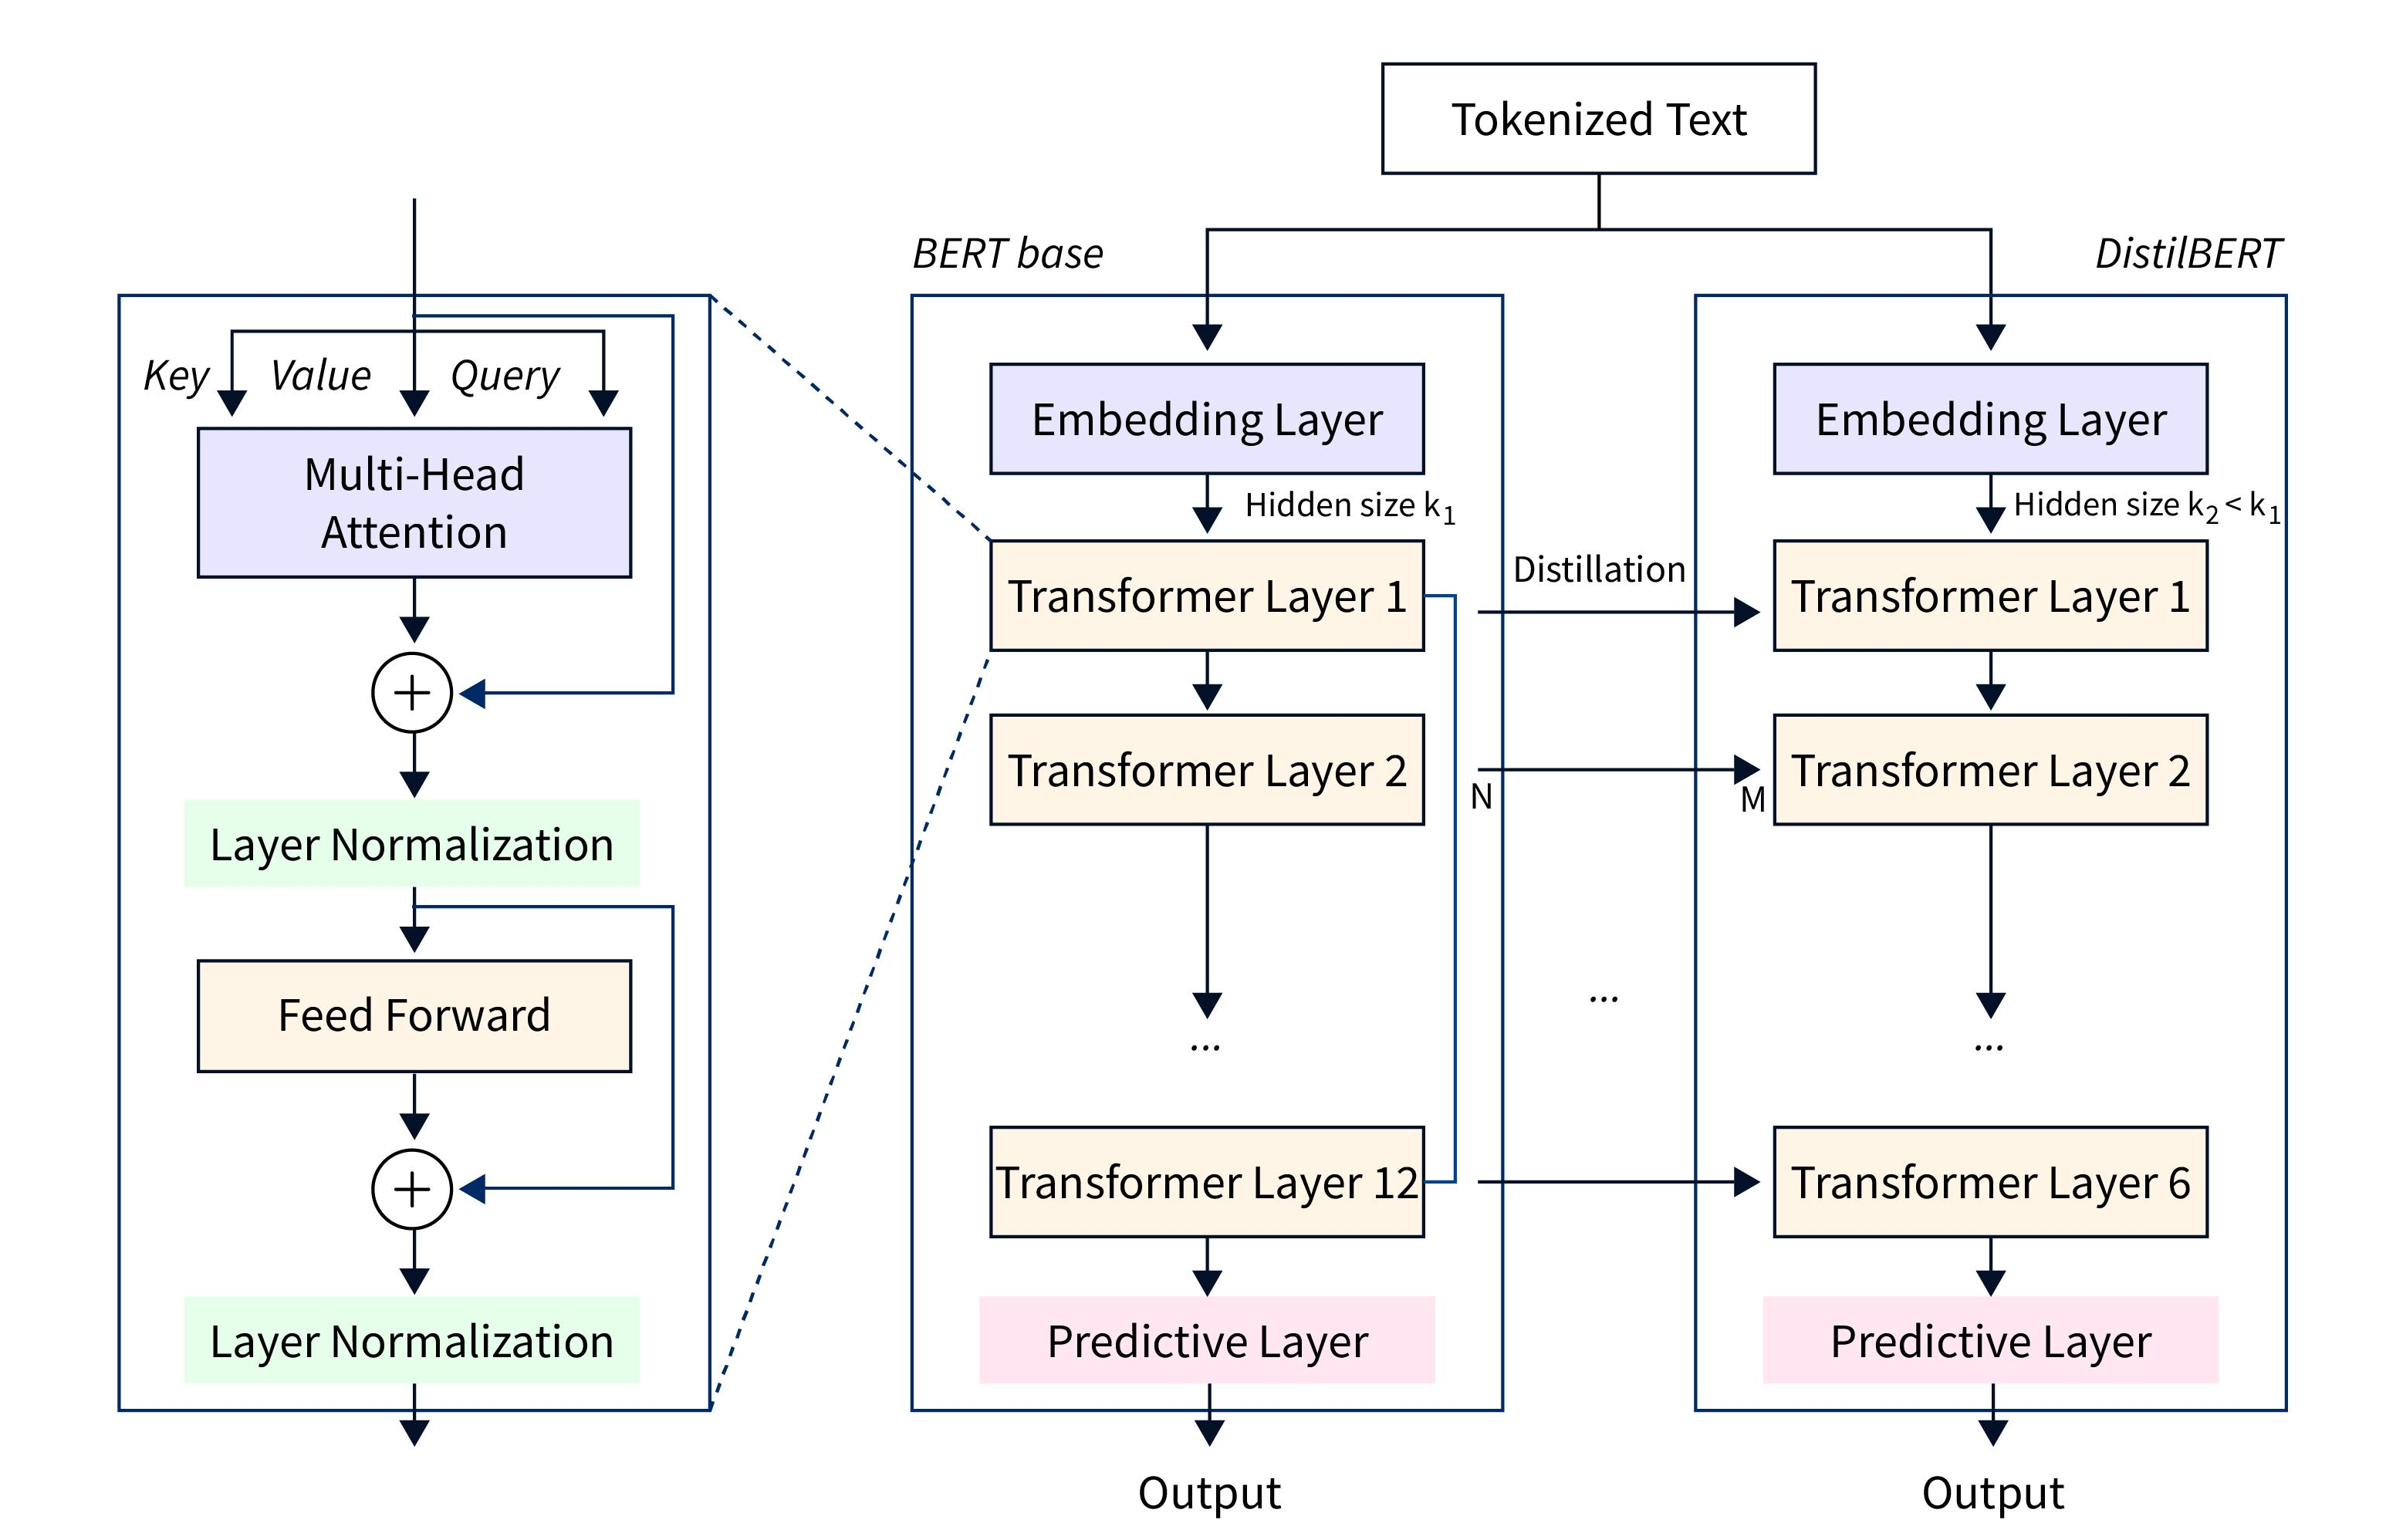
\includegraphics[width=1\linewidth]{figures/distilbert_architecture.png}
    \caption{Distilbert Architecture}
    \label{fig:distilbert_architecture}
\end{figure}

\subsubsection{Input Representation}
The input to the classifier is a tokenized string of the form:
\begin{Verbatim}[fontsize=\footnotesize]
[CLS] <surrounding HTML context> [SEP] <injection position marker> [SEP]
\end{Verbatim}
The surrounding HTML context is extracted from the page HTML around the injection point using BeautifulSoup: the 100 characters before and 100 characters after the injected probe string are taken, limited to the containing HTML element. The injection position marker is a description string generated from the reflection analysis (e.g., 'inside attribute value double-quoted' or 'inside script block string literal'). The combined input is truncated to 512 tokens using the DistilBERT tokenizer with WordPiece tokenization. Padding is applied to a fixed sequence length of 256 tokens for batch training efficiency.

\subsubsection{Training Methodology}
The classifier is fine-tuned on the labeled context classification dataset using the following training configuration:

\begin{table}[h]
    \centering
    \begin{tabular}{|p{2.7cm}|p{4cm}|p{7.3cm}|}
      \hline
        Hyperparameter & Value  &Rationale \\
         \hline
        Optimizer &AdamW  & Weight decay regularization; standard for transformer fine-tuning\\ \hline
         Learning rate&2e-5  &Recommended range for BERT-family models; prevents catastrophic forgetting
 \\ \hline
         LR scheduler&Linear warmup + cosine decay  & 5\% warmup steps; prevents early training instability\\ \hline
         
         Batch size & 32 (gradient accumulated) &Effective batch of 32; balances memory and gradient noise \\ \hline
         
         Epochs &10 with early stopping (patience 3)  & Prevent overfitting; restore best checkpoint\\ \hline
         Loss function & Cross-entropy &Prevent overfitting; restore best checkpoint \\ \hline
         Dropout &0.1 (inherited from DistilBERT)  & Regularization in attention and FFN layers\\ \hline
         Max\textcolor{white}{\_\allowbreak }sequence length& 256 tokens & Covers majority of injection contexts without padding overhead
\\
    \hline
    \end{tabular}
    \caption{DistilBERT Fine-Tuning Hyperparameters}
    
\end{table}

\subsubsection{Training Dataset}
The context classification dataset was constructed from three sources: 
\begin{enumerate}
    \item manually labeled injection contexts from a purpose-built testbed of vulnerable web applications
    \item synthetic examples generated by inserting probe strings into HTML scraped from the Common Crawl dataset
    \item examples from public XSS challenge write-ups where the injection context is described. The final dataset contains approximately 18,000 labeled examples distributed across eight classes, with balanced sampling to mitigate class imbalance.
\end{enumerate}

\subsubsection{Model Evaluation}

The model is evaluated on a held-out test split using accuracy, per-class precision, recall, and F1- score. The confusion matrix reveals the model's primary failure mode: confusion between semantically similar contexts. In practice, this confusion has minimal impact on scanner effectiveness because payloads suitable for quoted attribute contexts are a superset of those suitable for unquoted contexts.

\subsection{API design and Contract}

\subsubsection{REST API Specification}
\textbf{Authentication}\\
All API endpoints (except /health) require authentication via the x-api-key HTTP header or the Authorization: Bearer <key> header. The API key is compared using timing-safe comparison (crypto.timingSafeEqual) against the SHA-256 hash of API\_\allowbreak KEY\_\allowbreak SECRET stored in environment configuration. If API\_\allowbreak KEY\_\allowbreak SECRET is unset, the API operates in open/development mode with all authentication bypassed.

\textbf{Endpoint Specifications:} 
\lstset{
    basicstyle=\ttfamily\scriptsize,
    frame=single,
    breaklines=true,
    columns=fullflexible,
    keepspaces=true
}

\begin{lstlisting}[language=JavaScript, showstringspaces=false]
POST /scan -- Create and Enqueue a New Scan

Request Body:
{
  {
  "url": "https://target.example",
  "options": {
    "depth": 3,
    "maxParams": 100,
    "verifyExecution": true,
    "wafBypass": true,
    "maxPayloadsPerParam": 50,
    "timeout": 60000,
    "reportFormat": "\"["html", "json"],
    "singlePage": false,
    "auth": {
      "enabled": true,
      "loginUrl": "https://target.example/login",
      "username": "alice",
      "password": "secret",
      "usernameSelector": "input"\"[name=\\"username\\"]",
      "passwordSelector": "input"\"[name=\\"password\\"]",
      "submitSelector": "button"\"[type=\\"submit\\"]",
      "postLoginWaitMs": 3000,
      "successUrlContains": "/dashboard"
    }
  }
}
}

Response 201 Created:
{
  "scanId": "uuid-v4",
  "status": "QUEUED",
  "createdAt": "2026-05-01T12:00:00Z"
}
\end{lstlisting}

\begin{lstlisting}[language=JavaScript, showstringspaces=false]
GET /scan/:id -- Retrieve Scan Status and Results
Response 200:
{
  "id": "uuid",
  "targetUrl": "https://example.com",
  "status": "RUNNING",
  "phase": "FUZZ",
  "progress": 67,
  "vulnerabilities": [{
    "id": "vuln-uuid",
    "url": "https://example.com/search?q=",
    "parameter": "q",
    "payload": "<img src=x onerror=alert(1)>",
    "context": "HTML_BODY",
    "severity": "HIGH",
    "confidence": "CONFIRMED",
     \end{lstlisting}
      \begin{lstlisting}[language=JavaScript, showstringspaces=false]
    "cvssScore": 6.1
  }],
  "stats": {
    "urlsDiscovered": 45,
    "parametersScanned": 23,
    "payloadsSent": 412,
    "vulnerabilitiesFound": 3
  }
}
\end{lstlisting}

\textbf{WebSocket Protocol}
\\
The WebSocket server uses Socket.io with the default path '/socket.io'. Clients authenticate by passing the API key as a query parameter: $ws://host:3000/socket.io?apiKey=<key>$. After connection, clients join a scan-specific room by emitting join-scan with the scan ID:
\begin{lstlisting}[language=JavaScript, showstringspaces=false]
// Client join
socket.emit('join-scan', { scanId: 'uuid' });
// Server confirmation
socket.on('joined', ({ scanId }) => { ... });
// Progress update
socket.on('scan:progress', ({
 scanId, phase, progress, message
}) => { ... });
// Real-time finding
socket.on('scan:finding', ({
 scanId, vulnerability
}) => { ... });
\end{lstlisting}
\subsubsection{Python Service API Contracts}
\textbf{Context Module (/analyze)}

The Context Module is a FastAPI service running on port 5001. It exposes `POST /analyze` and `GET /health`.The implemented request model is:

\begin{lstlisting}[language=JavaScript]
{
  "url": "https://target.example/search?q=test",
  "params": \["q"],
  "waf": "none"
\end{lstlisting}
The implemented response is a parameter map:
\begin{lstlisting}[language=JavaScript]
{
  "q": {
    "reflects\_in": "html\_body",
    "allowed\_chars": \["<", ">", "\\""],
    "context\_confidence": 0.94
  }
}
\end{lstlisting}
The module injects markers into parameters, checks whether markers are reflected, determines context using regex, DOM parsing, and AI classification when available, and fuzzes allowed special characters. When the classifier artifact is unavailable, the service must not be described as fully DistilBERT-backed; it exposes `ai\_model\_loaded` through `/health`.

\textbf{Payload-Gen Module (/generate)}\\
The Payload-Gen module accepts classified injection points with context and WAF evasion flags, and returns a sorted list of payload objects. Each payload object includes the payload string, its context suitability, mutation type applied, and estimated success score from the ranker model.
\\ \\
\textbf{Fuzzer Module (/fuzz)}
The Fuzzer/Fuzzification module accepts injection targets with payload lists and scan options (timeout, concurrency). It returns a list of finding objects, each containing the injection details, HTTP evidence, browser verification result, and severity classification.
